\section{GeoFit Corrections on muon \pt}
\label{sec:geofitcorr}
In CMS, the reconstructed particle tracks can be displaced from the primary \textit{pp} interaction vertex. This displacement can be measured by transverse and longitudinal impact parameters denoted by d0 and z0 respectively. These parameters are used in differentiating particle tracks originating from the primary vertex (\textit{prompt}) from the tracks originating from a secondary vertex such as in b-quark decays. Muon selections that are used in this analysis guarantee that the d0 values of the muons are close to zero. However, it is possible to have small but non-zero d0 values. The effect of this residual d0 is observable as a trend in reconstructed \pt values of these muons, which in turn leads to a increase in reconstructed dimuon invariant mass resolution. This effect is corrected in both data and MC by \textit{GeoFit Corrections} that are derived in Z+jets MC samples, which uses muon d0 values calculated by using the beam spot information (\dzeroBS). Fig.~\ref{fig:dimu_mass_vs_d0} shows the trend in reconstructed dimuon mass when plotted against $\text{d0}_{\text{BS,}\mu^+}$ before and after the corrections. The corrections improve the dimuon mass resolution in both data and MC without introducing an overall mass scale shift or any other bias. Fig.~\ref{fig:ggH_dimu_mass_geofit} shows dimuon mass distributions for ggH signal MC before and after the \textit{GeoFit Corrections}. The details of \textit{GeoFit Corrections} can be found in Section~\ref{sec:app_geofitcorr}.


\begin{figure}[h!]
    \centering
    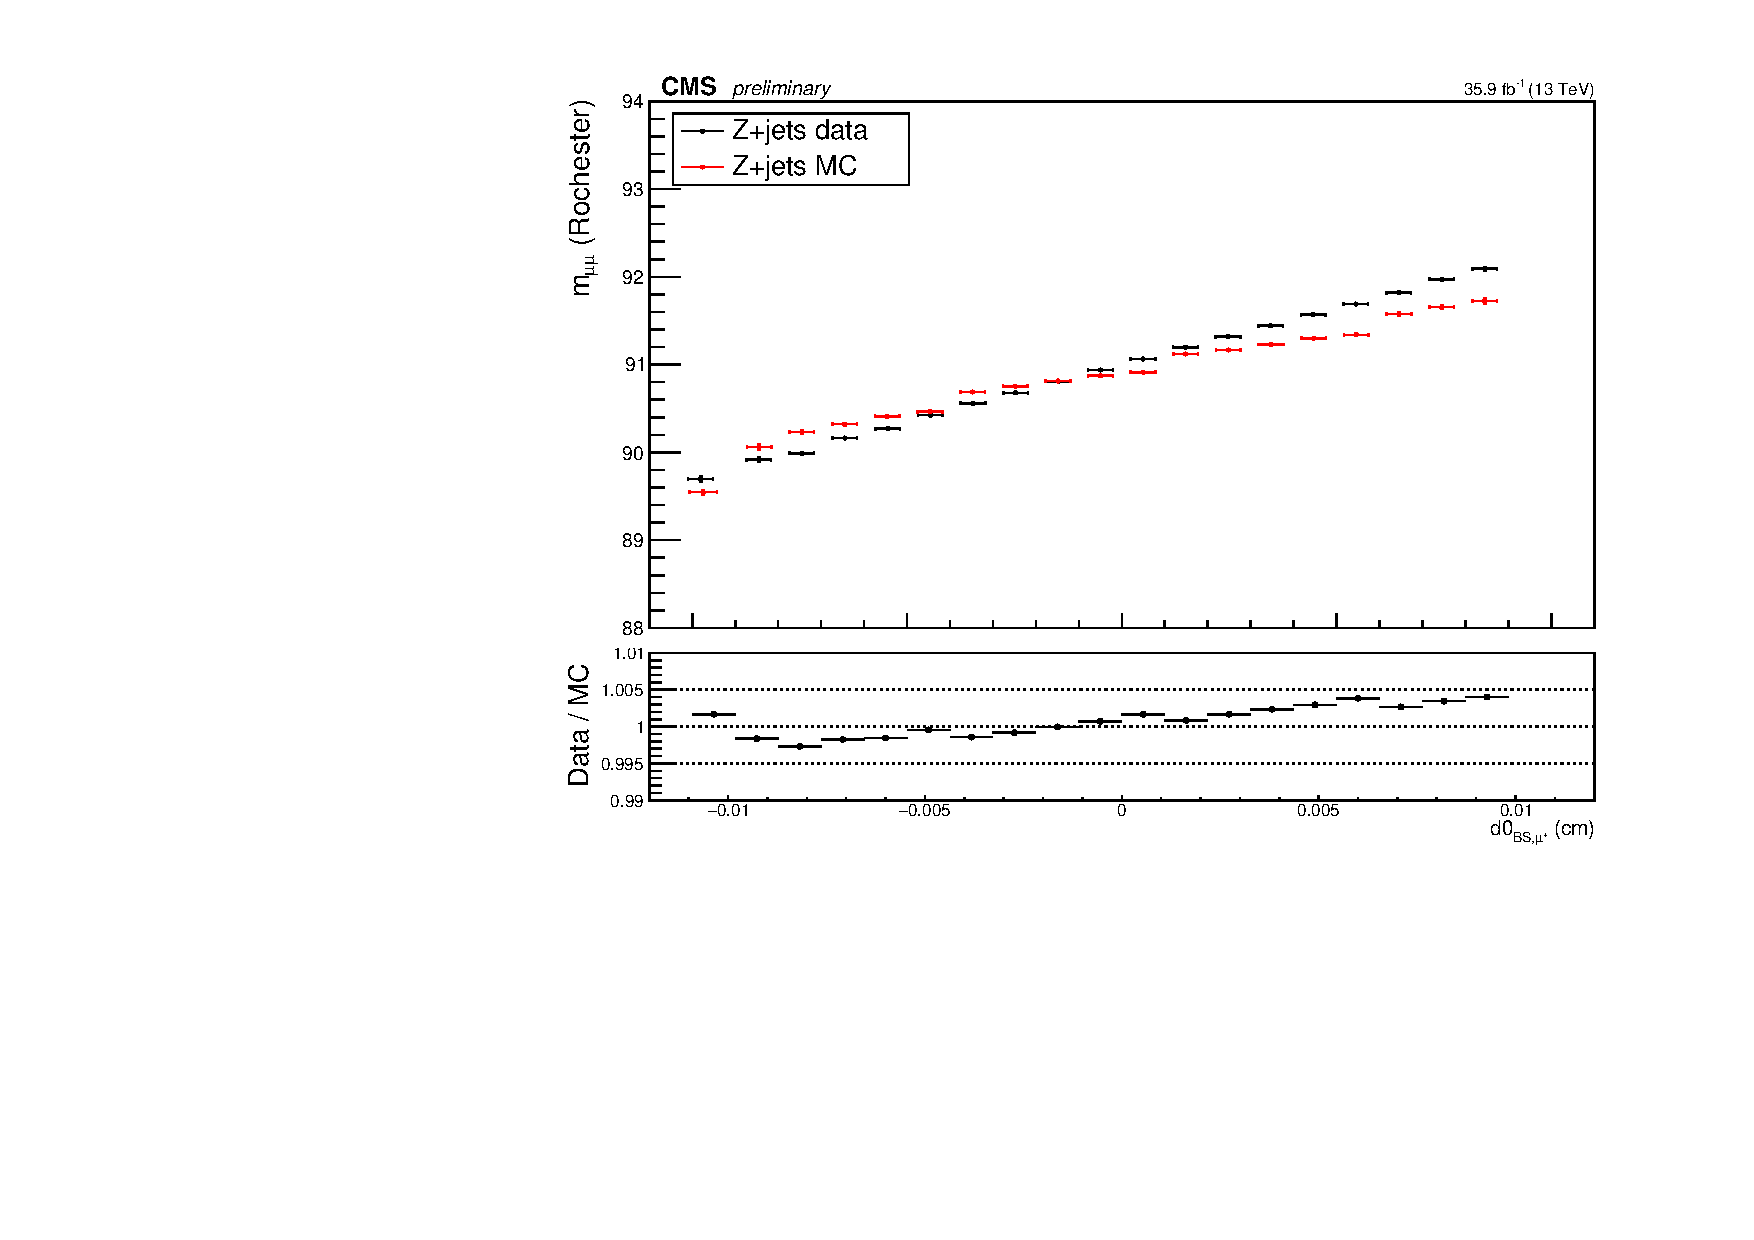
\includegraphics[width=0.49\textwidth]{images_geofit/dimu_mass_vs_d0BS_Roch.pdf}
    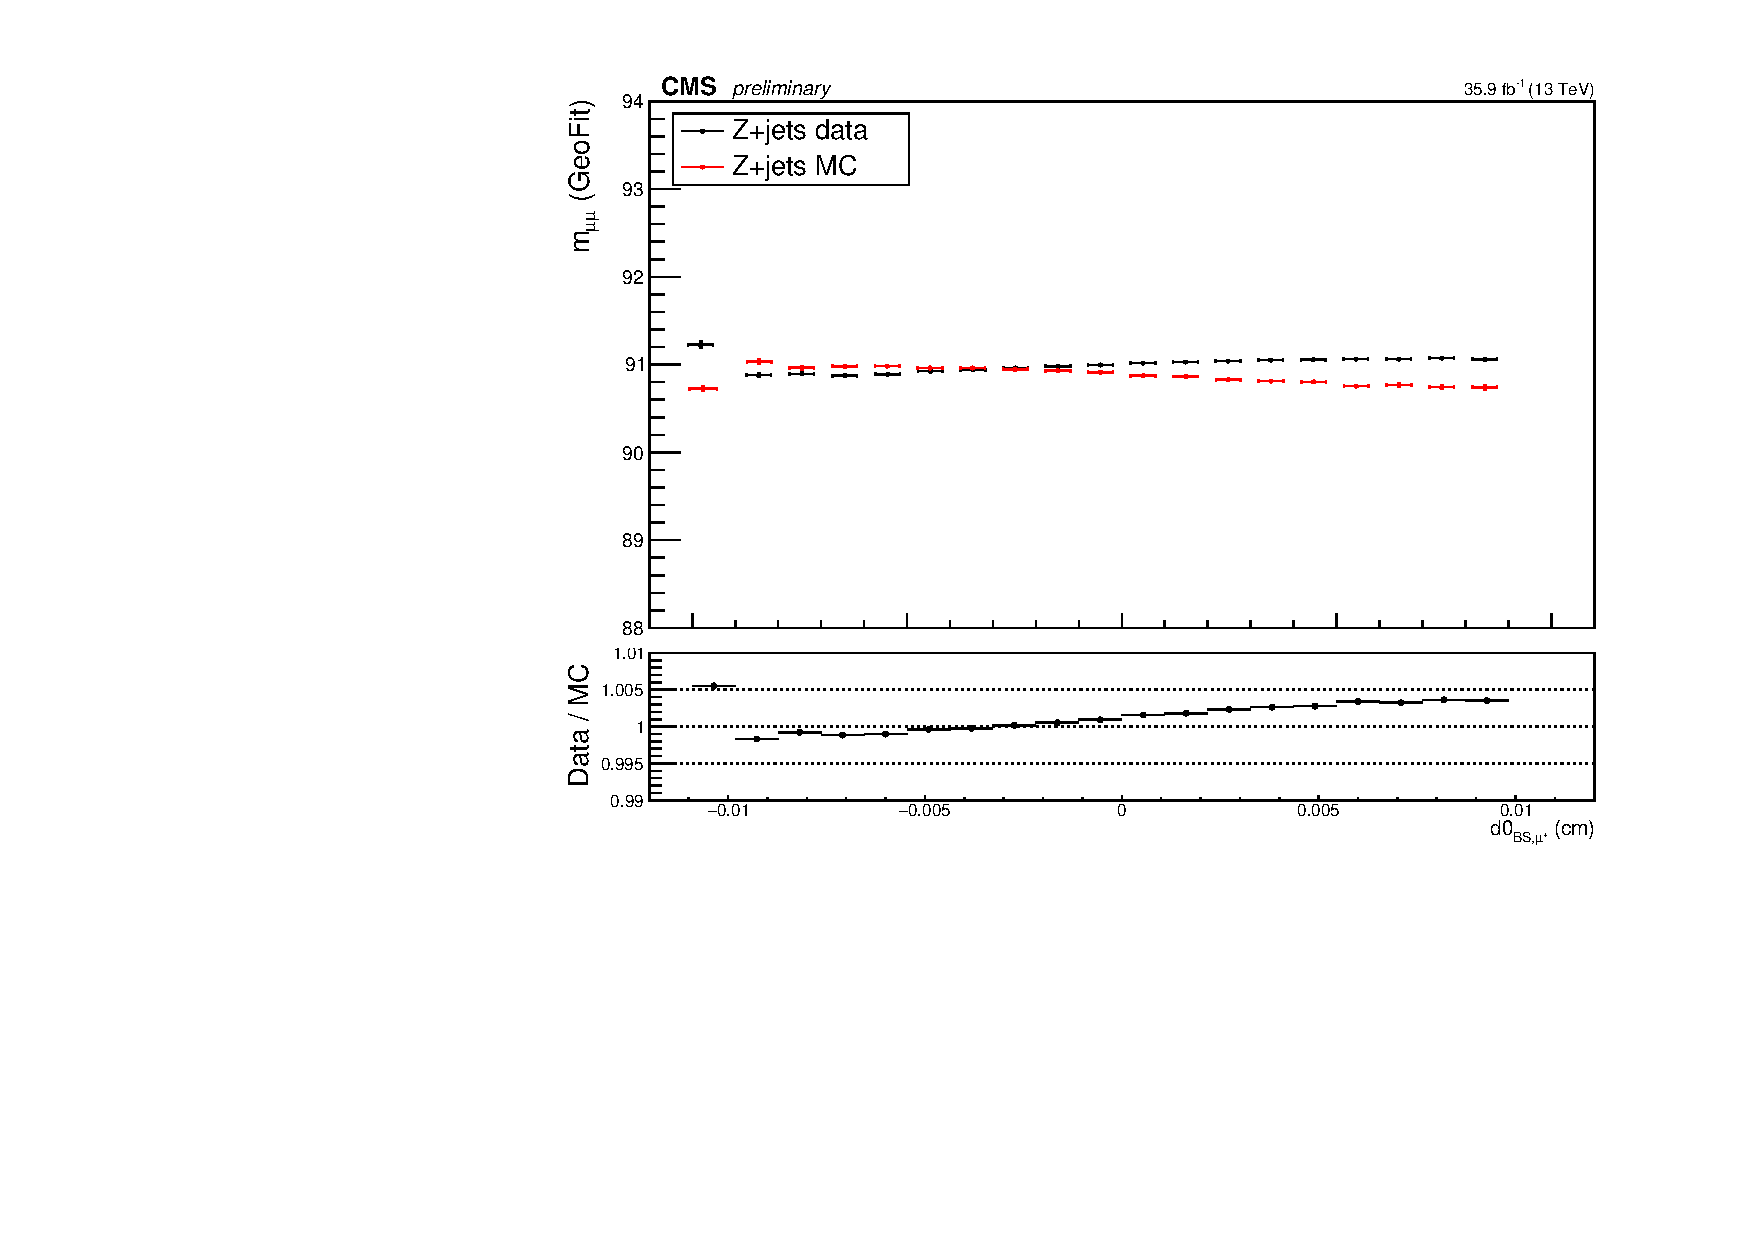
\includegraphics[width=0.49\textwidth]{images_geofit/dimu_mass_vs_d0BS_geofit.pdf}
    \caption{Dimuon mass peak mean value vs. $\text{d0}_{\text{BS,}\mu^+}$ before (left) and after (right) \textit{GeoFit Corrections} showing in 2016 Z+jets data and MC.}
    \label{fig:dimu_mass_vs_d0}
\end{figure}


\begin{figure}[h!]
    \centering
    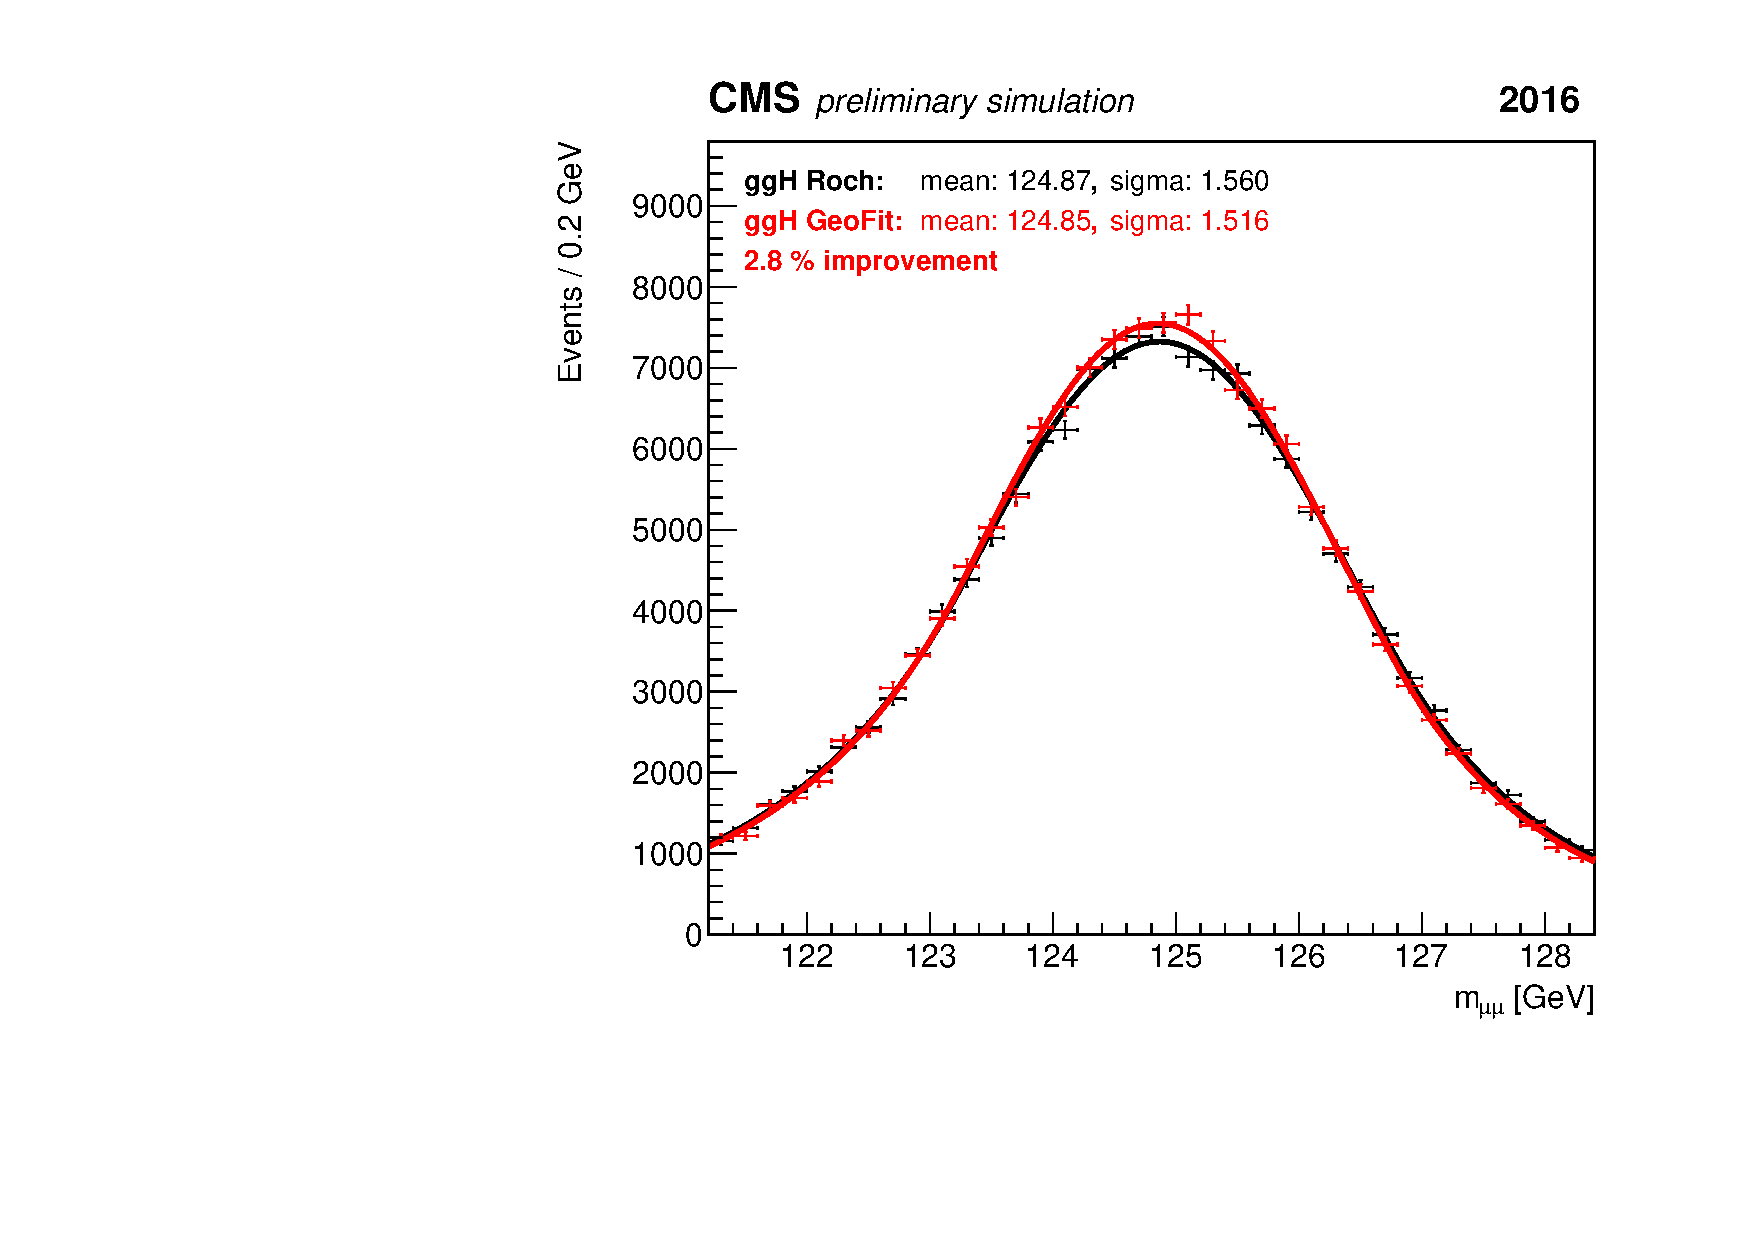
\includegraphics[width=0.32\textwidth]{images_geofit/ggH_mass_geofit_2016.pdf}
    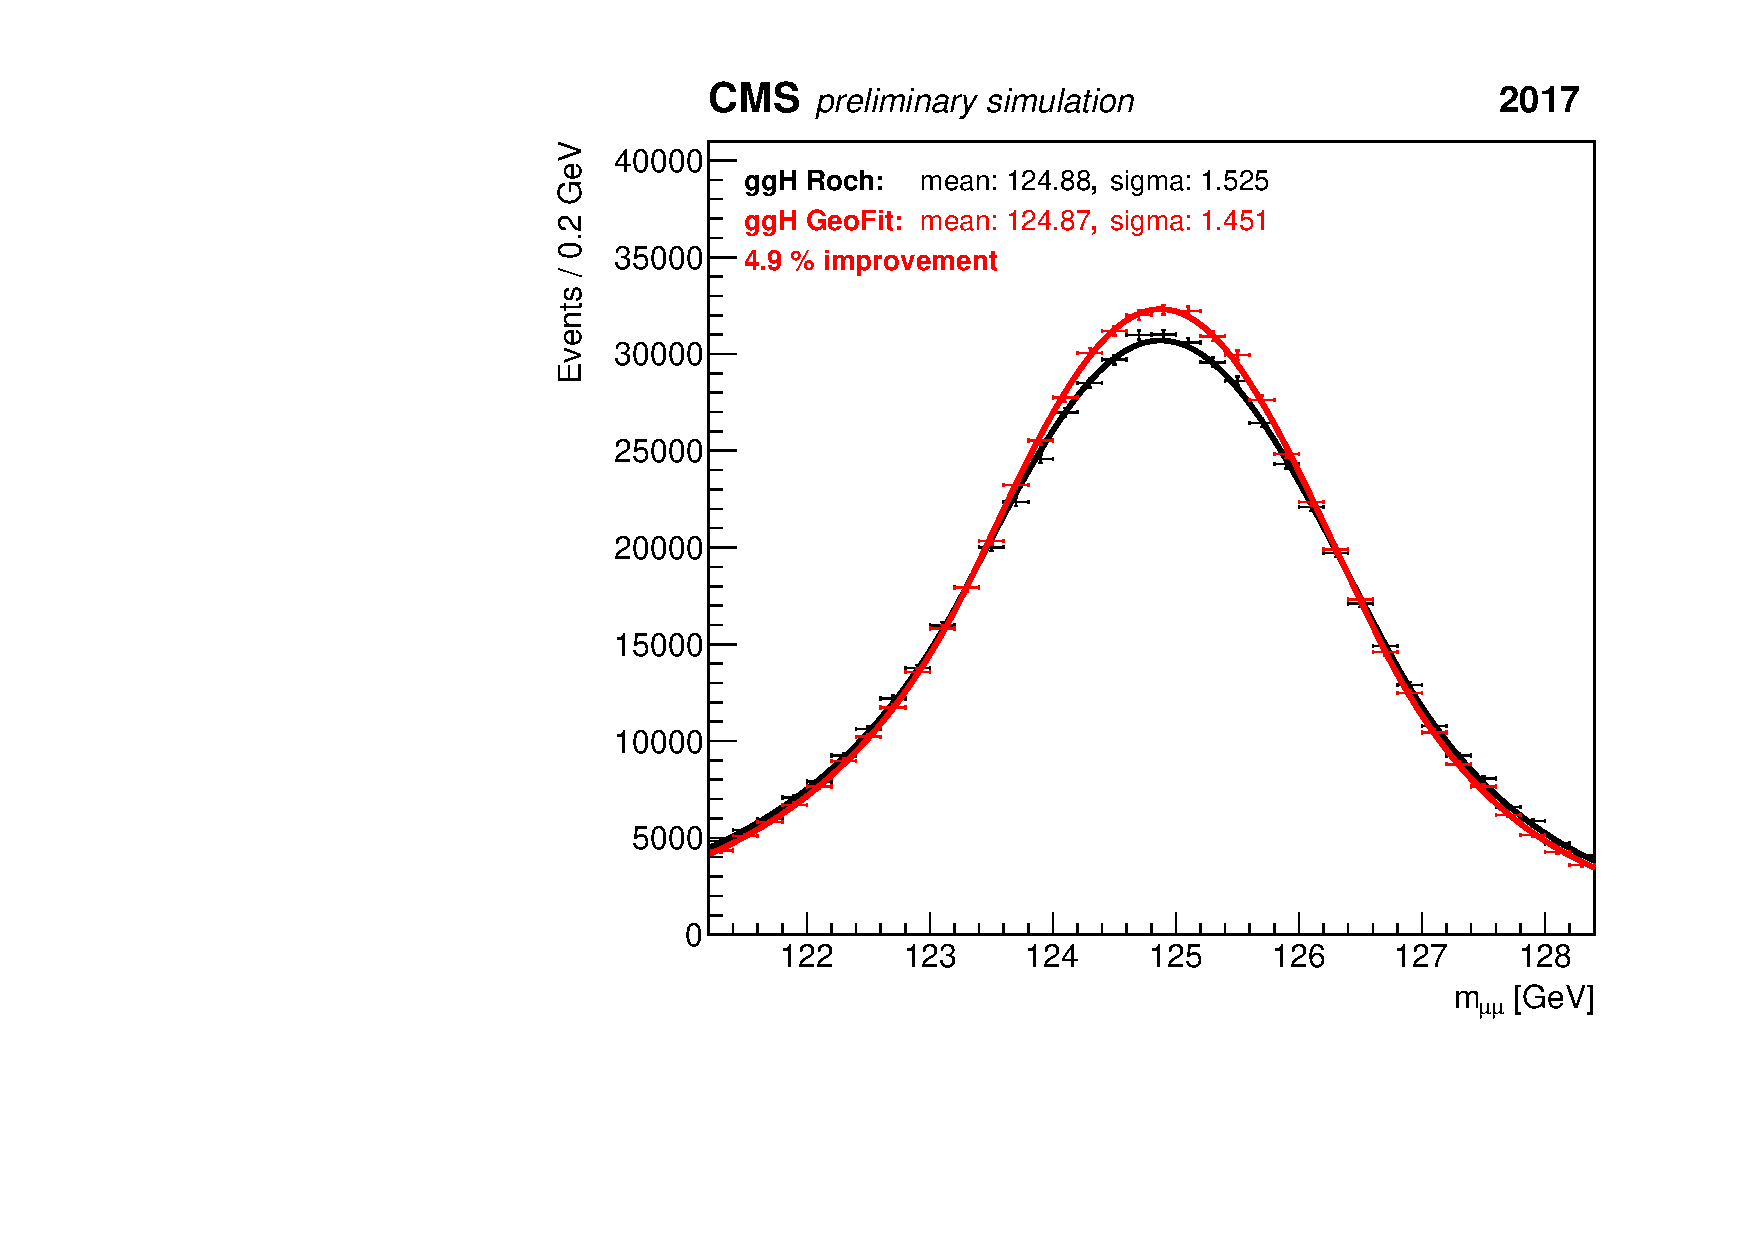
\includegraphics[width=0.32\textwidth]{images_geofit/ggH_mass_geofit_2017.pdf}
    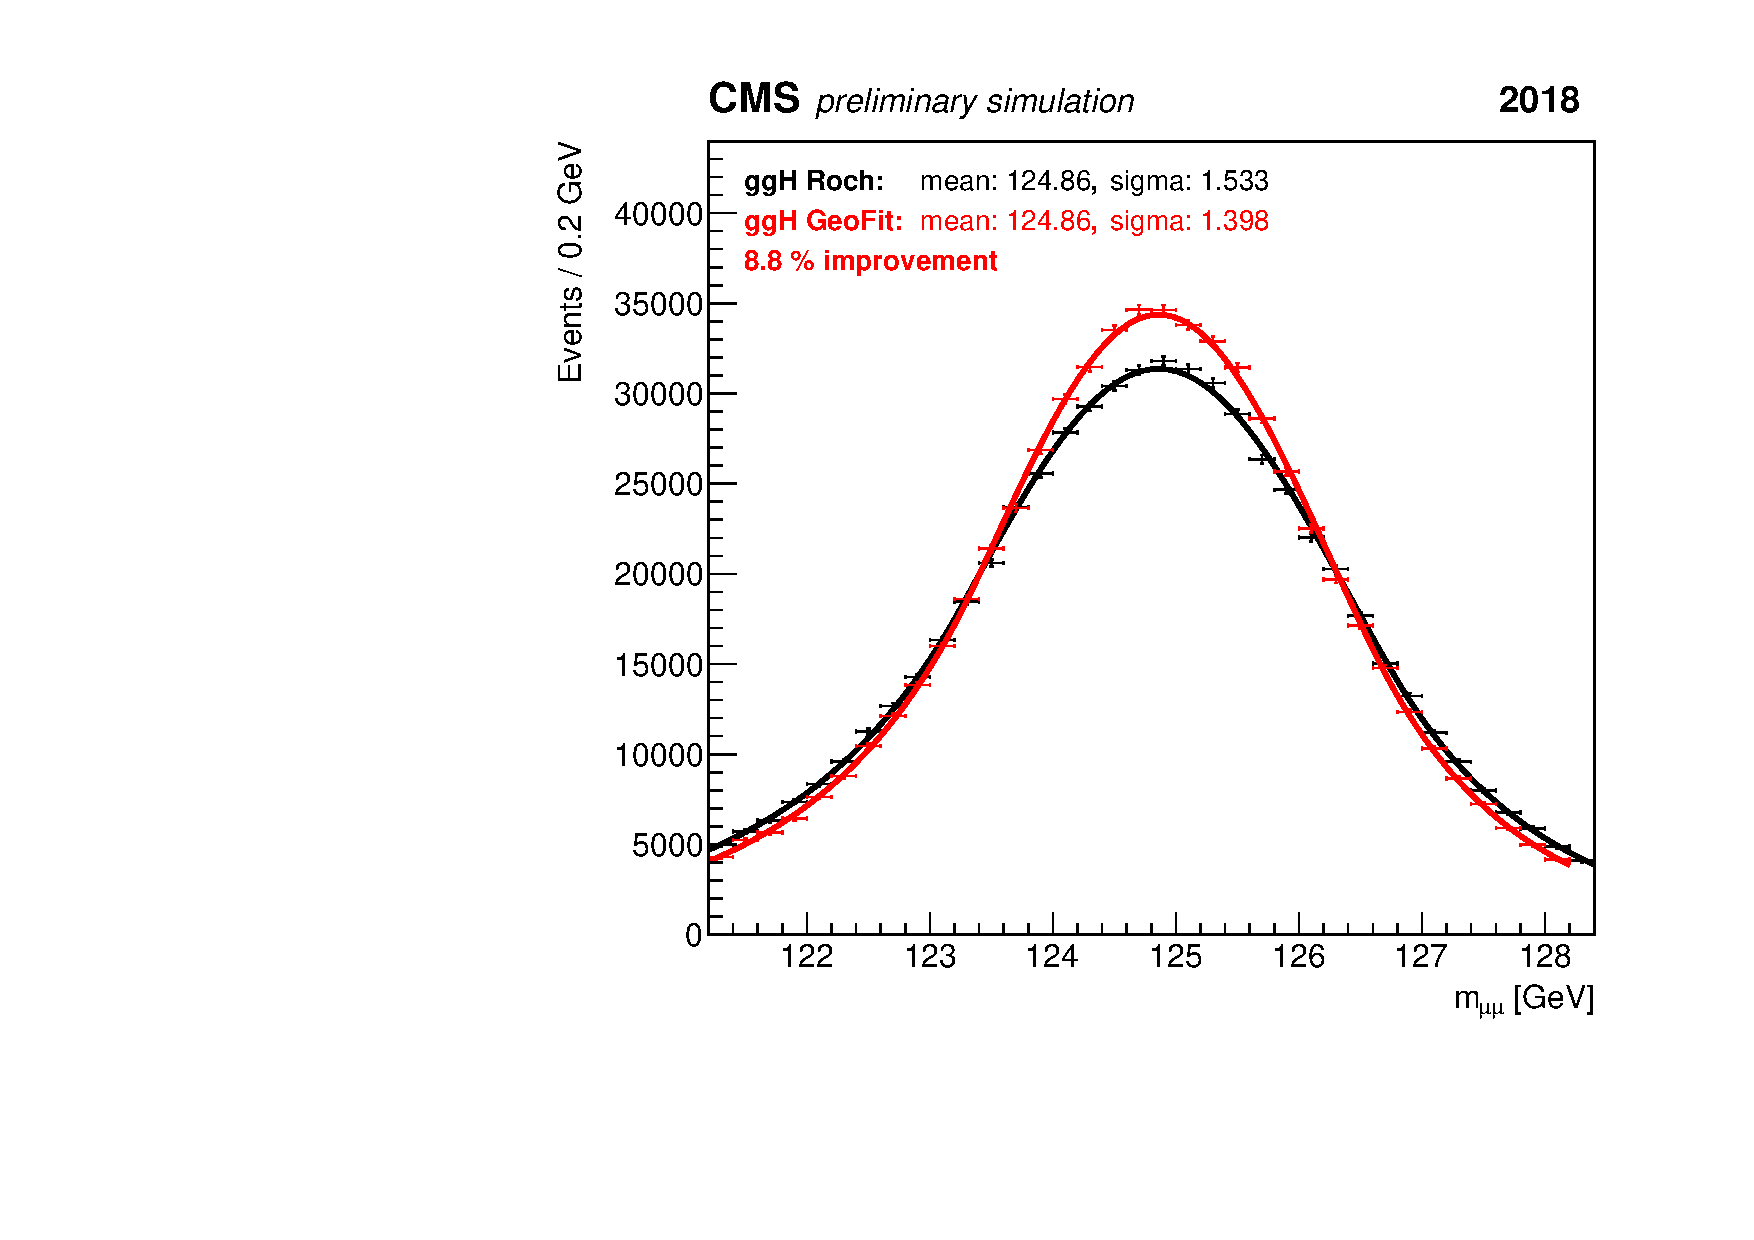
\includegraphics[width=0.32\textwidth]{images_geofit/ggH_mass_geofit_2018.pdf}
    \caption{Dimuon mass peak around 125 \gev for ggH signal MC samples in 2016 (left), 2017 (center) and 2018 (right) fitted by using a double-sided crystal ball function.}
    \label{fig:ggH_dimu_mass_geofit}
\end{figure}





